\documentclass[12pt]{article}

\usepackage{setspace}
\usepackage{lipsum}
\usepackage{graphicx}
\usepackage[table,xcdraw]{xcolor}
\usepackage{hyperref}

\title{Evaluation of Nonparametric Bayesian Classification Methods for Predicting Fake News from Article Titles}
\author{Nathaniel Hawkins}
\date{}

\begin{document}
	\maketitle
	
	\section{Introduction}
	
    It is growing increasingly important to remain up to date with current events in our modern-day political climate. The proliferation of ``fake news'' as a term for slander has cast doubt on media and news sources alike, making it challenging for individuals to distinguish between the true sources of information, and borderline propaganda meant to lower the popular opinion of a particular candidate. It is, therefore, important for checks and systems to lie in place that can quickly and accurately determine whether or not the information one is consuming is legitimate. In this work, we will evaluate two nonparametric Bayesian classification methods, k-nearest neighbors (KNN) and Parzen window (PW), for their ability to distinguish between real news and ``fake news.'' We will compare these nonparametric methods to a suite of baselines classifiers in the scikit-learn (sklearn) python library. Through these efforts, we hope to not only contribute to the field of fake news detection, but answer two major questions: 1) how accurately can this prediction task be done using the title of the news article alone?, and 2) how well do nonparametric methods perform compared to some popular and simple classifiers?
    
    The field of fake news detection has largely been dominated by deep-learning-based methods\cite{oshikawa:2020}. The field largely began making progress starting in 2017 following major progress in the field of deep learning in general\cite{bhatt:2017}. A wide variety of deep learning methods have been implemented for classifying fake news. These include fully connected deep networks\cite{thota:2018,saikh:2020}, long short term memory networks \cite{rodriguez:2019, kumar:2020}, bi-directional long short term memory networks \cite{popat:2018,qawasmeh:2019,abedalla:2019,kumar:2020}, convolutional neural networks \cite{rodriguez:2019, kumar:2020}, graph convolutional neural networks\cite{monti:2019}, recurrent neural networks\cite{girgis:2018, singhania:2017}, and sophisticated language-based models like BERT\cite{abedalla:2019, zellers:2019}. These models have achieved variable success in classifying fake news with accuracies topping out well over 98\%. While these methods are highly accurate and complex, the time required to train and implement these models is substantial. The hardware and time requirements for training and utilizing these models often exceeds that available to the typical user. Additionally, as more training data becomes available, retraining and reiplementing these methods quickly becomes infeasible. Therefore, these ``simpler'' models, while traditionally achieving lower performances comparably\cite{oshikawa:2020}, are easier to implement, easier to retrain, and much less computationally costly. The features used in the classification task have also widely ranged. They have included continuous bag of words representations, TF-IDF vectorizations, and neural network embeddings like ELMo and GloVe. In this work, we will evaluate the effectiveness of nonparametric models on the simplest feature set: a one-hot encoding of the article titles. While a one-hot encoding of article titles is less linguistically informative compared to something like a neural network embedding, it allows us to focus the prediction task on the first thing a reader would see (i.e., the title) and further reduces computational time by making the feature space sparser. Though, we note that using more robust feature sets, including the contents of the article itself, pose an area of future work for this project.
	
    \section{Data}
    
    To carry out this work, we utilized a publicly available dataset on Kaggle. The dataset can be found by \href{https://www.kaggle.com/clmentbisaillon/fake-and-real-news-dataset}{clicking this text}. The features of this dataset is summarized in Table \ref{table:1}. The news articles range from early 2015 to mid 2018. Predominantly, the topics of these articles are political news and world news, which addresses the motivation behind this work well. There is a slight class imbalance present in this data with approximately 1,000 more fake news articles than true news articles. This class imbalance is negligible compared to the total number of samples (approximately 1-2\%), but we will address this issue using class-balanced 5-fold cross validation and averaging the performance across folds. By doing so, the imbalance will be ``averaged'' out and we project it will not significantly impact performance. 

    %% Begin Table Summarizing Datas5et
    \begin{table}
    \begin{center}
        \begin{tabular}{|c|c|}
            \hline
            \textbf{Number of Article Titles}&44,266\\
            \hline
            \textbf{Number of Article Titles (True)}&21,416\\
            \hline
            \textbf{Number of Article Titles (Fake)}&22,850\\
            \hline
            \textbf{Mean Length of Titles (Words)}&9.29\\
            \hline
            \textbf{Median Length of Titles (Words)}&9\\
            \hline
            \textbf{Minimum Length of Titles (Words)}&1\\
            \hline
            \textbf{Maximum Length of Titles (Words)}&29\\
            \hline
            \textbf{Number of Features After One-Hot Encoding}&18,206\\
            \hline
        \end{tabular}
        \caption{Summary of dataset used in this work. Lengths shown in this table are the texts following preprocessing.}
        \label{table:1}
    \end{center}  
    \end{table} 	
    
     %% Histogram of title lengths
    \begin{figure}[htbp]
        \centerline{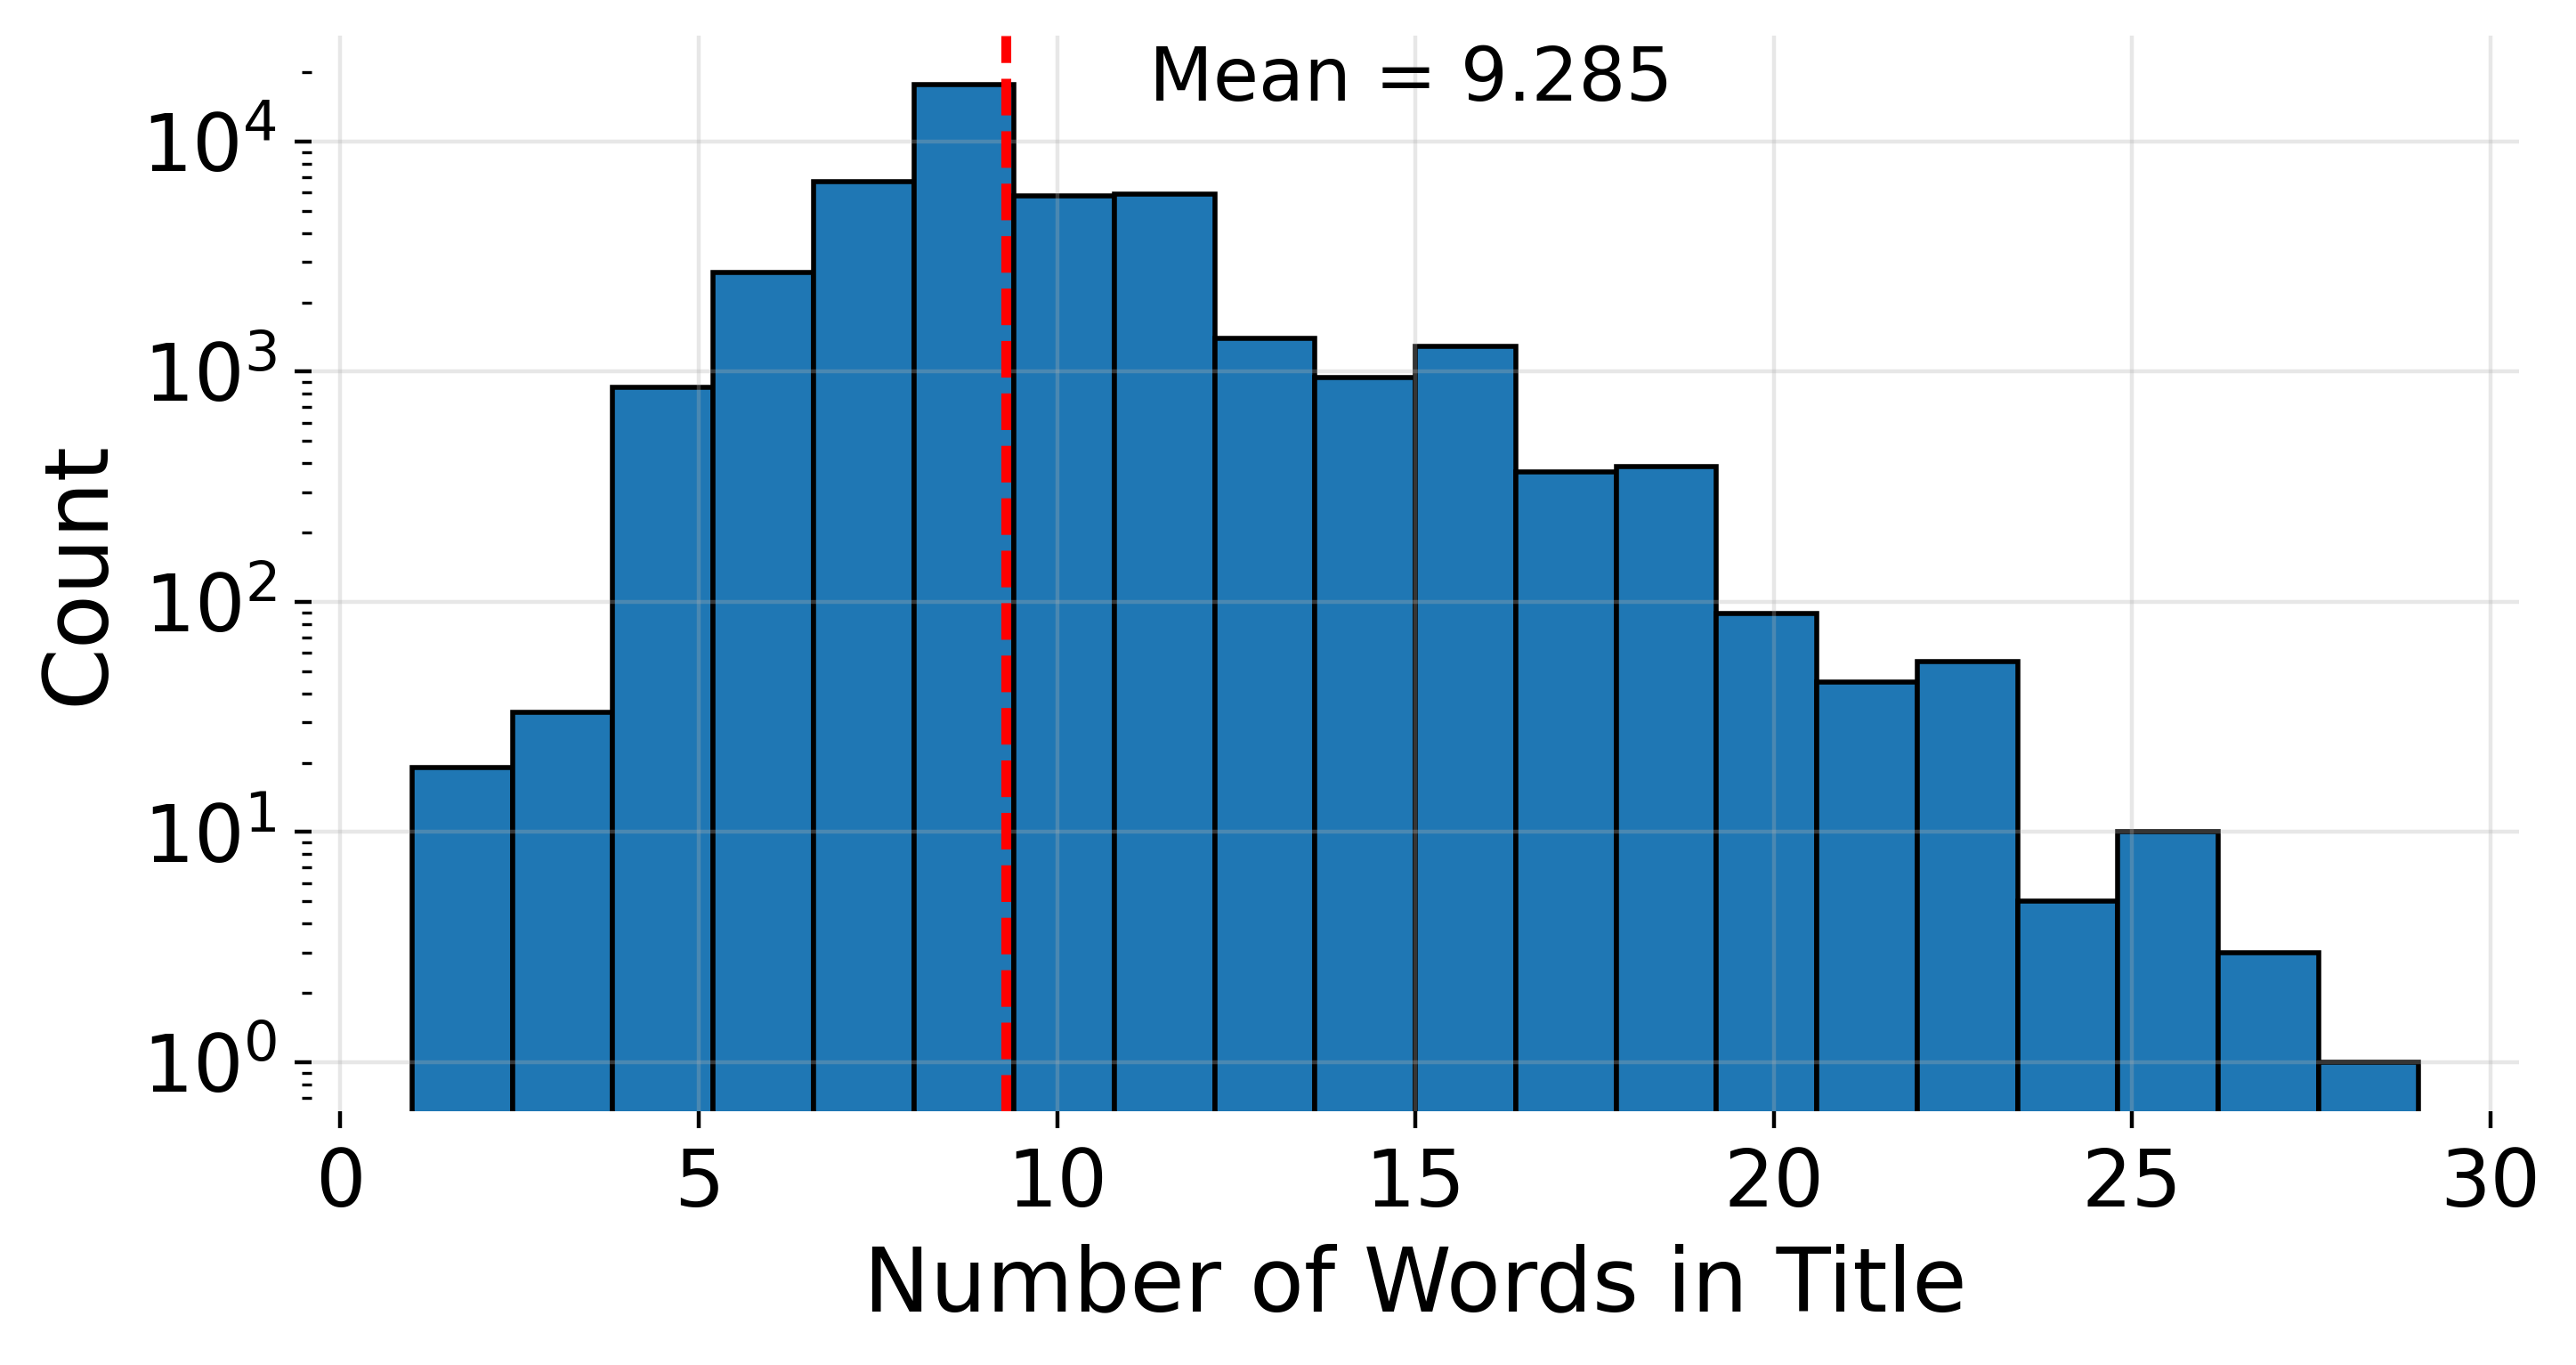
\includegraphics[scale=1]{../results/length_of_description.png}}
        \caption{Histogram of length of article titles. Mean description shown with verticle red line. Y-axis is logarithmically scaled.}
        \label{fig:1}
\end{figure}	
	
	\section{Methods}
	
    Prior to training our classifiers, we first preprocessed the titles of the articles before vectorizing them to create our feature set. The preprocessing follows most of the standard steps used in other works\cite{oshikawa:2020}. We first extracted all of the titles from the dataframe for fake and true news. Then, we removed non-UTF-8 enocdable characters, removed punctuation from the titles using regular expressions, filtered out stopwords (e.g., ``at,'' ``and,'' ``the,'') using the list of english stopwords in the NLTK python library, and stemmed the text using the Porter stemming algorithm in NLTK. Text preprocessing is a staple for most NLP tasks because it removes language artifacts and casts the words into a more general form. In the case of this works, the text preprocessing reduces the dimensionality of the final feature space once we vectorize it. The preprocessed article titles are cast to numerical representations by turning them to one-hot vectors. The size of the vector is equal to the total number of unique words across all titles in the corpus. Each index corresponds to a single word. To vectorize a title, the feature vector gets a value of 1 if the word is present at all in that title (no matter how many times) and a 0 if it is not. This vectorization is done using the \texttt{feature\_extraction.text.CountVectorizer(binary = True)} function in sklearn. 
	
	The baseline models used in this work are all implemented in sklearn. The baseline models are described in Table \ref{table:2}. For this work, we chose some of the most widely used classifiers in the sklearn library. We implemented two supper vector machine classifiers, one using a linear kernel and one using the radial basis function, logistic regression, multiplayer perceptron, and naive bayes as our baselines. All classifiers use the default parameters used by sklearn. In this way our baseline models are not optimized classifiers with finely tuned hyperparameters. 
	
	We used the sklearn implementation of KNN as it is more computationally efficient than what we could implement. For PW, we created a simple implementation (see \texttt{parzen.py}). Our implementation of PW follows the algorithm outlined in class. To evaluate these nonparametric methods, we wanted to test a wide variety of hyperparameters. For KNN, tested with $k=$3,5,7,9,11,13,15,17,19, and 21, and for PW, we tested $h =$ 0.01,0.05,0.1,0.5,1,5,10, and 50.
	
    For evaluation metrics, we report the accuracy score, area under the precision recall curve (auPRC), area under the receiver operator curve (auROC), F1 score (F1) and the computation time. We chose to report all of these metrics because each details a difference aspect of the classifiers. Accuracy and auROC give a broad description of the classifier and are the most widely used classifier metrics, but they are insensitive metrics when class imbalances are present. As noted, the imblanace here is comparatively minimal, but we want to include metrics which are more sensitive to imbalances. Therefore, we also include auPRC and F1, which take into account both precision and recall. Computation time is reported to give an idea of the cost associated with using these classifiers. Reported metrics are averaged over 5-fold cross validation. Class balance is maintained across 5-fold cross validation to ensure representative training. 
		
	

	\section{Results}
	
    The results for our baselines are shown in Table \ref{table:2}. The KNN and PW results are shown in Table \ref{table:3} and \ref{table:4}, respectively. A plot showing performance versus computation time is shown in Figure \ref{fig:2}.
    
    %% Baselines
    \begin{table}[]
    \centering
    \begin{tabular}{|c|c|c|c|c|c|}
    \hline
    \textbf{Method} & \textbf{Accuracy} & \textbf{auPRC} & \textbf{F1} &                             \textbf{auROC} & \textbf{Time} \\ \hline
    \textbf{Linear SVM} & 0.95 & 0.92 & 0.95 & 0.95 & 19752.63 \\ \hline
    \textbf{Log Reg}    & 0.95 & 0.92 & 0.95 & 0.95 & 126.59   \\ \hline
    \textbf{MLP}        & 0.94 & 0.90 & 0.93 & 0.94 & 1506.45  \\ \hline
    \textbf{NB}         & 0.80 & 0.71 & 0.82 & 0.80 & 21.52    \\ \hline
    \textbf{RBF SVM}    & 0.95 & 0.93 & 0.95 & 0.95 & 25225.82 \\ \hline
    \end{tabular}
    \caption{Baseline model results averaged over 5-fold cross validation. Times shown are in seconds. Linear SVM: sklearn implementation of support vector classifier (SVC) with default parameters using a linear kernel. Log Reg: sklearn implementation with default parameters. MLP: sklearn implementation of multilayer perceptron with default parameters. NB: sklearn implementation of naive bayes classifier with default parameters. RBF SVM: sklearn implementation of SVC with default parameters using radial basis function as the kernel.}
    \label{table:2}
    \end{table} 
    
    
    %% KNN
    \begin{table}[]
    \centering
\begin{tabular}{|c|c|c|c|c|c|}
\hline
\textbf{Method} & \textbf{Accuracy} & \textbf{auPRC} & \textbf{F1} & \textbf{auROC} & \textbf{Time} \\ \hline
\textbf{KNN-3}  & 0.77 & 0.71 & 0.74 & 0.77 & 11176.50 \\ \hline
\textbf{KNN-5}  & 0.74 & 0.69 & 0.69 & 0.74 & 10014.54 \\ \hline
\textbf{KNN-7}  & 0.72 & 0.67 & 0.64 & 0.71 & 11483.15 \\ \hline
\textbf{KNN-9}  & 0.70 & 0.65 & 0.60 & 0.69 & 11389.89 \\ \hline
\textbf{KNN-15} & 0.68 & 0.64 & 0.55 & 0.67 & 10377.58 \\ \hline
\textbf{KNN-17} & 0.69 & 0.65 & 0.57 & 0.68 & 10979.94 \\ \hline
\textbf{KNN-19} & 0.70 & 0.66 & 0.58 & 0.69 & 10967.81 \\ \hline
\textbf{KNN-21} & 0.71 & 0.66 & 0.60 & 0.70 & 11090.60 \\ \hline
\end{tabular}
\caption{KNN results averaged over 5-fold CV.}
\label{table:3}
\end{table}
    
    %% Parzen Window
    \begin{table}[]
    \centering
    \begin{tabular}{|c|c|c|c|c|c|}
    \hline
    \textbf{Parzen $h$} & \textbf{Accuracy} & \textbf{auPRC} & \textbf{F1} &                             \textbf{auROC} & \textbf{Time} \\ \hline
    \end{tabular}
    \caption{}
    \label{table:4}
    \end{table} 
    
    %% Accuracy vs. Time
%    \begin{figure}[htbp]
%        \centerline{\includegraphics[scale=1]{}}
%        \caption{Accuracy versus time.}
%        \label{fig:2}
%\end{figure}
	
	\section{Discussion and Conclusions}
	
    
    
    %% Bibliography
    \newpage
    \nocite{*}
    \bibliography{report} 
    \bibliographystyle{ieeetr}
	
\end{document}
